%
% transdil.tex
%
% (c) 2019 Prof Dr Andreas Müller, Hochschule Rapperswil
%
\ifthenelse{\boolean{presentation}}{

\begin{frame}
\frametitle{Translation und Dilatation}
\begin{center}
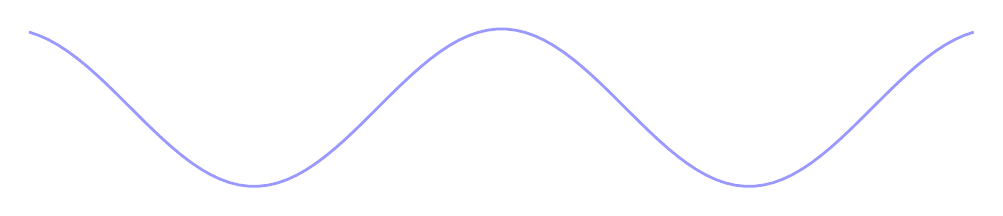
\begin{tikzpicture}[>=latex]

\draw[color=blue!40,line width=1pt] plot[domain=-6:6,samples=100]
	({\x},{1.1+cos(\x*(180/3.1415))-4});

\def\bmax{101}
\pgfmathparse{0.5*(\bmax-1)}
\xdef\s{\pgfmathresult}

\foreach \b in {1,...,{\bmax}}{
	\only<\b>{
		\pgfmathparse{6*((\b)-1-\s)/(\s)}
		\xdef\B{\pgfmathresult}
		\pgfmathparse{1.1+cos(\B*180/3.1415)}
		\xdef\A{\pgfmathresult}
		\flaeche{\A}{\B}{1}
		\achsen{1.5}
		\curve{\A}{\B}{1}
		\cwt{\A}{\B}{-2.0}
	}
}

\end{tikzpicture}
\end{center}
\end{frame}

}{}






